\setcounter{ExampleCounter}{1}
\marginnote{\includegraphics[scale=0.07]{Marathon1}}
If you were training for a marathon and you currently run 3 miles a day, you may choose to increase your distance by half a mile every week.  Can we predict how far you'll be running in six weeks, or how long it will take to reach your goal?  With small numbers like these, you could answer those questions without using an equation, but we'll use this as an example to show how to build a simple model from a scenario like this.

Let $P_t$ represent the number of miles that you run after $t$ weeks, so $P_0$ would be the number of miles you currently run, $P_1$ would represent the number of miles you run after 1 week, and so on.  We can define a \textbf{recursive relationship} like the following one to represent the scenario that was laid out.
\begin{align*}
P_0 &= 3\\
P_t &= P_{t-1} + 0.5
\end{align*}
A recursive relationship is one that relates the next value in a sequence to previous values.  We could use this relationship to go from $P_0$ to $P_1$ to $P_2$ and so on, all the way to $P_6$ to answer the first question, and we could keep going from one value to the next until we reached 26 to answer the second question.  However, this would be tedious and mindless, so instead we prefer an \textbf{explicit equation}, or closed-form equation.  Especially for predictions far into the future, the recursive form is impractical, even though it arises easily from the problem description.

In this case, the explicit form is pretty straightforward, but deriving it from the recursive form will be instructive:
\begin{align*}
P_0 &= 3\\
P_1 &= 3+0.5\\
P_2 &= 3+0.5+0.5 = 3+(0.5)2\\
P_3 &= 3+0.5+0.5+0.5 = 3 + (0.5)3\\
&\vdots\\
P_t &= 3 + 0.5t
\end{align*}

This explicit equation gives an easy way to quickly answer both questions.  We can substitute 6 for $t$ to find that $P_6 = 3+0.5(6) = 6$ miles, and we can substitute 26 for $P_t$ and solve for $t$ to find how long it'll take to reach your goal:
\begin{align*}
26 &= 3+0.5t\\
23 &= 0.5t\\
46 &= t
\end{align*}
It'll take 46 weeks to reach your goal.
\begin{center}
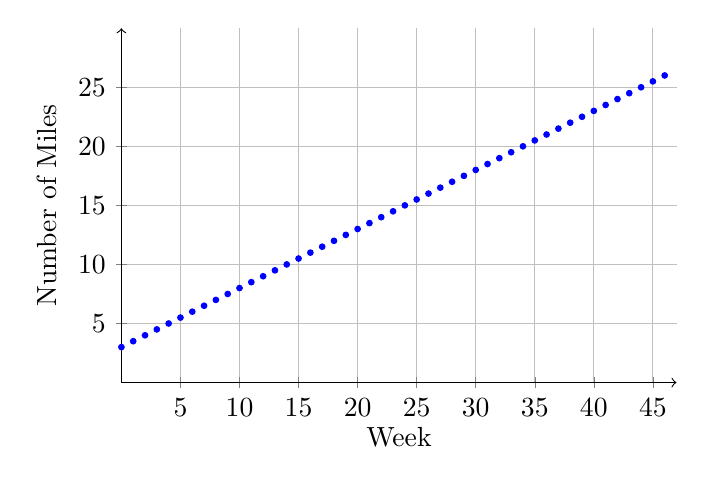
\begin{tikzpicture}
\begin{axis}[
    xmin=0, xmax=47,
    ymin=0, ymax=30,
    axis lines=center,
    axis on top=false,
    domain=0:1,
    x=0.15cm,
    y=0.15cm,
    xtick={5,10,...,45},
    xticklabels={5,10,...,45},
    ytick={0,5,...,25},
    yticklabels={0,5,10,15,20,25,30},
    axis lines=middle,
    axis line style={->},
    x label style={at={(axis description cs:0.5,-0.1)},anchor=north},
    y label style={at={(axis description cs:-0.1,.5)},rotate=90,anchor=south},
    xlabel={Week},
    ylabel={Number of Miles},
    grid=major
    ]
	\addplot [blue,only marks,mark size=1] table {
	0 3
	1 3.5
	2 4
	3 4.5
	4 5
	5 5.5
	6 6
	7 6.5
	8 7
	9 7.5
	10 8
	11 8.5 
	12 9
	13 9.5
	14 10
	15 10.5
	16 11
	17 11.5
	18 12
	19 12.5
	20 13
	21 13.5
	22 14
	23 14.5
	24 15
	25 15.5
	26 16
	27 16.5
	28 17
	29 17.5
	30 18
	31 18.5
	32 19
	33 19.5
	34 20
	35 20.5
	36 21
	37 21.5
	38 22
	39 22.5
	40 23
	41 23.5
	42 24
	43 24.5
	44 25
	45 25.5
	46 26
	};
	%\addplot [blue, thick] table {
	
	%};
\end{axis}
\end{tikzpicture}
\end{center}
%\begin{center}
%\includegraphics[width=0.8\textwidth]{LinearGraph1}
%\end{center}
This graph shows why we call this \textit{linear} growth.  If we graph the number of miles versus the week, the points lie along a straight line.

This is consistent for every problem where a number grows by a constant amount every time period.

\begin{formula}{Linear Growth}
If some quantity starts at size $P_0$ and grows by $d$ every time period, then the quantity after $t$ time periods can be determined using either of the following relations.\\

Recursive form:
\[P_t = P_{t-1}+d\]

Explicit form:
{\Large \[P_t = P_0 + dt\marginnote{This is the one we'll use in the rest of the examples in this section.}\]}

Here $d$ represents the common difference---the amount that the quantity changes each time $t$ increases by 1.

Notice that this could refer to linear growth or linear decay; if $d$ is negative, the quantity will decrease linearly.
\end{formula}

Knowing that the key to linear growth is this common difference between terms, we can recognize linear growth from data if each term is the previous term plus a constant.
\begin{center}
\begin{tabular}{p{0.5in} p{0.75in} p{1.25in}}
\textbf{Term} & \textbf{Quantity} & \textbf{Difference from Previous Term}\\
\hline
& & \\
0 & 15 & \\
1 & 27 & 12\\
2 & 39 & 12\\
3 & 51 & 12\\
4 & 63 & 12\\
5 & 75 & 12\\
\end{tabular}
\end{center}
As we can observe in this table, if we note that the quantity adds a constant amount each time, we know that the growth is linear, and we can write the closed-form equation given above.\\

Notice that this is exactly the standard linear equation that you've seen in your algebra classes:
\begin{align*}
y &= mx+b\\
P_t &= dt + P_0
\end{align*}
Here, $P_0$ is the $y$-intercept, since it is the starting point, and thus the value when $t=0$.  Also, $d$ is the slope here, or the amount by which the quantity changes when $t$ increases by 1.

These two equations are the same, but as you'll see when modeling, we often rename the pieces to more closely match the names of the real-world quantities we're measuring.

\begin{example}[https://www.youtube.com/watch?v=cpaNK4jbMkA]{Elk Population}
The population of elk in a national forest was measured to be 12,000 in 2011 and 15,000 in 2015.  If the population continues to grow linearly at this rate, what do we expect the elk population to be in 2022?\\

\marginnote{\includegraphics[scale=0.07]{Elk1}}
We first need to define the parts of our linear growth equation.  The initial amount $P_0$ is the amount when $t=0$, but we won't use the actual year 0 as our starting point.  Instead, the initial amount in this problem is given in 2011, so we'll define $t=0$ to be the year 2011, so $P_0=12,000$.\\

Next we need to find $d$, the growth per time period.  Since the time period in this example is one year, we'll need to find how much the population grew each year.
\begin{center}
\begin{tabular}{c c}
\textbf{Year} & \textbf{Population}\\
\hline
0 & 12,000\\
4 & 15,000
\end{tabular}
\end{center}
Since the population grew by 3,000 in 4 years, this represents a growth of 3,000/4 = 750 per year.  Thus $d=750$.\\

Note that this is equivalent to using the slope formula: $\dfrac{\textrm{rise}}{\textrm{run}}$
\[d = \textrm{ slope } = \dfrac{\textrm{change in population}}{\textrm{change in time}} = \dfrac{15,000 - 12,000}{2015 - 2011} = \dfrac{3000}{4} = 750\]

Now we can write the explicit equation that models this population growth:
\[P_t = 12,000 + 750t\]

To answer the question, we note that 2022 corresponds to $t=11$, since 2022 is 11 years after 2011.
\[P_{11} = 12,000 + 750(11) = 20,250 \textrm{ elk}\]
\end{example}

\begin{try}[http://www.izzomath.com/103text/growthmodels/example1.1/story.html]
If we estimated the population of trout in a pond to be 2200 in 2008 and 3500 in 2012, construct a linear model to predict the population in 2017.
\end{try}
\vspace{0.5in}

Now let's try an example with data that is nearly linear, but not exactly.
\begin{example}[https://www.youtube.com/watch?v=QoOdfeLBN0o]{Gasoline Consumption}
Gasoline consumption in the US has been increasing steadily.  Data from 1995 to 2004 is shown below.  Find a linear model for this data, and use it to predict consumption in 2018.  If the trend continues, when will consumption reach 200 billion gallons?\\

\marginnote{\includegraphics[scale=0.16]{GasTanker1}}
\begin{center}
\begin{tabular}{|p{1in} | c | c | c | c | c | c | c | c | c | c|}
\hline
\textbf{Year} & '95 & '96 & '97 & '98 & '99 & '00 & '01 & '02 & '03 & '04\\
\hline
\textbf{Consumption (billions of gallons)} & 116 & 118 & 119 & 123 & 125 & 126 & 128 & 131 & 133 & 136\\
\hline
\end{tabular}
\end{center}

If we plot this data, it appears to have an approximately linear relationship.
\begin{center}
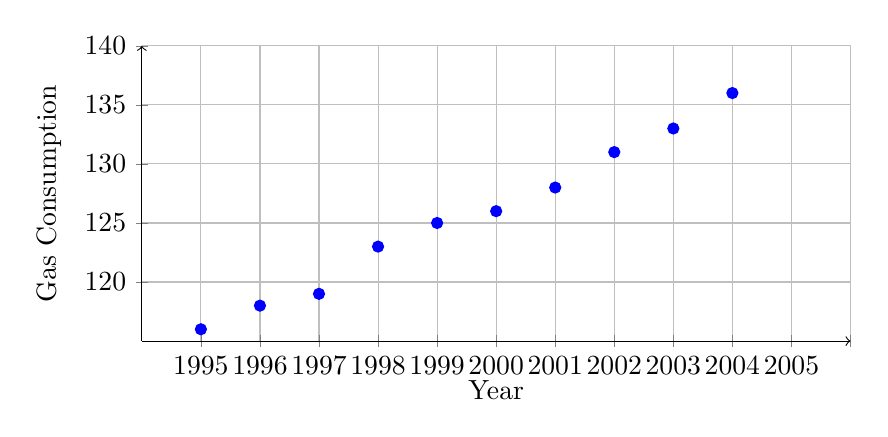
\begin{tikzpicture}
\begin{axis}[
    xmin=0, xmax=12,
    ymin=0, ymax=25,
    axis lines=center,
    axis on top=false,
    domain=0:1,
    x=0.75cm,
    y=0.15cm,
    xtick={0,1,...,12},
    xticklabels={1994,1995,1996,1997,1998,1999,2000,2001,2002,2003,2004,2005},
    ytick={0,5,...,25},
    yticklabels={115,120,125,130,135,140},
    axis lines=middle,
    axis line style={->},
    x label style={at={(axis description cs:0.5,-0.1)},anchor=north},
    y label style={at={(axis description cs:-0.1,.5)},rotate=90,anchor=south},
    xlabel={Year},
    ylabel={Gas Consumption},
    grid=major
    ]
	\addplot [blue,only marks] table {
	1 1
	2 3
	3 4
	4 8
	5 10
	6 11
	7 13
	8 16
	9 18
	10 21
	};
	%\addplot [blue, thick] table {
	
	%};
\end{axis}
\end{tikzpicture}
\end{center}
%\begin{center}
%\includegraphics[width=0.8\textwidth]{LinearGraph2}
%\end{center}

While we could use a statistical technique known as \textit{linear regression} to find an equation to model the data, we can find a simple model by using just two pieces of data to calculate an average change.  We'll use the data from 1995 and 2004 for this.\marginnote{We could use the data from any two years to calculate the slope (and we would get slightly different answers), but a common convention is to use the first and last years.  You should follow this convention when answering the homework questions.}
\begin{center}
\begin{tabular}{c | c}
\textbf{Year} & \textbf{Consumption}\\
\hline
1995 & 116\\
2004 & 136
\end{tabular}
\end{center}

\begin{align*}
d &= \textrm{ slope } = \dfrac{\textrm{change in consumption}}{\textrm{change in time}} = \dfrac{136 - 116}{2004 - 1995} = \dfrac{20}{9}\\
&= 2.22 \textrm{ billion gallons per year}
\end{align*}
\vfill
\pagebreak

Now we can write our model:
\[P_t = 116 + 2.2t\]
\begin{center}
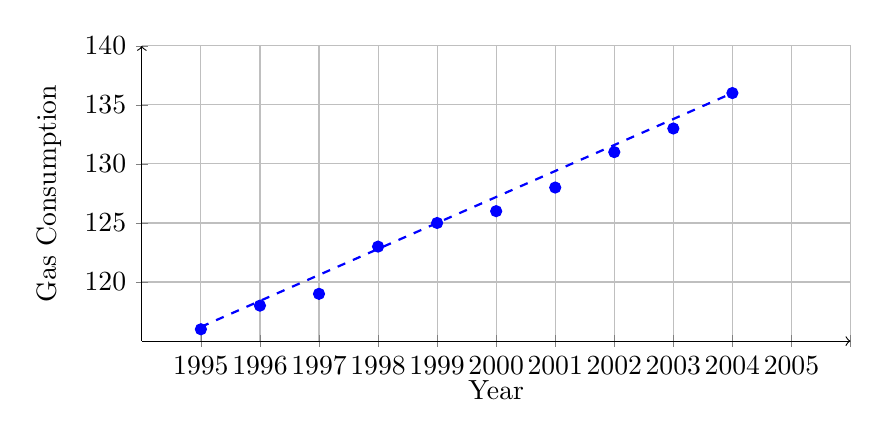
\begin{tikzpicture}
\begin{axis}[
    xmin=0, xmax=12,
    ymin=0, ymax=25,
    axis lines=center,
    axis on top=false,
    domain=0:1,
    x=0.75cm,
    y=0.15cm,
    xtick={0,1,...,12},
    xticklabels={1994,1995,1996,1997,1998,1999,2000,2001,2002,2003,2004,2005},
    ytick={0,5,...,25},
    yticklabels={115,120,125,130,135,140},
    axis lines=middle,
    axis line style={->},
    x label style={at={(axis description cs:0.5,-0.1)},anchor=north},
    y label style={at={(axis description cs:-0.1,.5)},rotate=90,anchor=south},
    xlabel={Year},
    ylabel={Gas Consumption},
    grid=major
    ]
	\addplot [blue,only marks] table {
	1 1
	2 3
	3 4
	4 8
	5 10
	6 11
	7 13
	8 16
	9 18
	10 21
	};
	\addplot [blue, thick,dashed,domain=1:10] {2.2*x-1};
\end{axis}
\end{tikzpicture}
\end{center}
%\begin{center}
%\includegraphics[width=0.8\textwidth]{LinearGraph3}
%\end{center}

Now we can use our model to make predictions about the future, using the simplifying assumption that the previous trend continues unchanged.
\begin{itemize}
\item Predicting gas consumption in 2018, when $t=23$:\marginnote{This example illustrates the two main types of questions that we often want to answer:\\ \text{}\\
1. Predicting the value of what we are measuring at a given point in time.\\ \text{}\\
2. Predicting the point in time when the thing we are measuring will reach a certain value.}
\[P_{23} = 116 + 2.2(23) = 166.6\]
Our model predicts that the US will consume 166.6 billion gallons of gasoline in 2018 if the current trend continues.

\item Predicting when consumption reaches 200 billion gallons:
\begin{align*}
200 &= 116 + 2.2t\\
84 &= 2.2t\\
38.18 &= t
\end{align*}
This model predicts that gas consumption will reach 200 billion gallons about 38 years after 1995, or the year 2033.
\end{itemize}
\end{example}

\begin{try}[http://www.izzomath.com/103text/growthmodels/example1.1/story.html]
The number of stay-at-home fathers in Canada has been growing steadily at an approximately linear rate.  Use the data from the table below to find an explicit formula for the number of stay-at-home fathers and use it to predict the number in 2020.  Use 1976 and 2010 to find the average rate of change.
\begin{center}
\begin{tabular}{|p{1.25in} | c | c | c | c | c|}
\hline
\textbf{Year} & 1976 & 1984 & 1991 & 2000 & 2010\\
\hline
\textbf{Number of stay-at-home fathers} & 20,610 & 28,725 & 43,530 & 47,665 & 53,555\\
\hline
\end{tabular}
\end{center}
\end{try}

Again, we understand that this model is not perfect; the US will most likely not consume exactly 166.6 billion gallons of gas in 2018, but we expect consumption to be \textit{about} that.  In practice, we'll often make predictions and then compare them to actual measured results to assess the accuracy of our model.  A very simple linear model like this will likely have fairly large error; more sophisticated models tend to have smaller errors.

\begin{example}[https://www.youtube.com/watch?v=3GG3aOIc9Pk]{Gym Membership Cost}
The cost, in dollars, of a gym membership for $t$ months can be described by the explicit equation
\[P_t = 70 + 30t.\]
What does this equation tell us?\\

\marginnote{\includegraphics[scale=0.07]{Gym1}}
The value for $P_0$ in this equation is 70, so the initial cost is \$70, which means that there must be a sign-up fee of \$70 to join the gym.\\

The value for $d$ in the equation is 30, so the cost increases by \$30 each month, which means that the monthly membership fee for the gym is \$30 a month.
\end{example}

\subsection{When Good Models Go Bad}
When predicting the future with mathematical models, it is crucial to keep in mind that few trends continue indefinitely.

\begin{example}[https://www.youtube.com/watch?v=7_wAlvsCyDc]{A Boy's Height}
Suppose a four year old boy is currently 39 inches tall, and you are told to expect him to grow 2.5 inches a year.\\

We can set up a growth model, with $t=0$ corresponding to 4 years old.
\[P_t = 39 + 2.5t\]

At six years old (when $t=2$), we would expect him to be
\[P_2 = 44 \textrm{ inches tall},\]
but this model eventually breaks down.  Certainly, we shouldn't expect him to grow at the same rate all his life.  If he did, at age 50 he would be
\[P_{46} = 154 \textrm{ inches } = 12.8 \textrm{ feet tall}.\]
\end{example}

Of course, this boy will not grow at a constant rate, but rather experience growth spurts and ultimately stop growing in his early 20s.  But this example also illustrates that we should check our model against common sense.
\vspace{0.5in}

Let's look at another example that illustrates the need for a common sense check.

\begin{example}[https://www.youtube.com/watch?v=3FeV7lvkATI]{Marathon Times}
The table below shows the record times for the marathon for men and women from 1965 to 1980.
\begin{center}\marginnote{\includegraphics[scale=0.07]{WomanRunner1}}
\begin{tabular}{l | c | c}
\textbf{Year} & \textbf{\color{blue}Men's Times (min)} & \textbf{\color{orange!70!black}Women's Times (min)}\\
\hline
& & \\
1965 & 132 & \\
1966 & & \\
1967 & 129.5 & 195\\
1968 & & \\
1969 & 128.5 & \\
1970 & 129.5 & 183\\
1971 & & 175\\
1972 & & \\
1973 & & 166\\
1974 & 129 & 163\\
1975 & & 158\\
1976 & & \\
1977 & & 155\\
1978 & 129 & 152\\
1979 & & 147\\
1980 & 129 & 145\\
\end{tabular}
\vspace{0.5in}

We can plot these data points, and the graph below shows the men's times in blue and the women's times in orange.
\vfill
\pagebreak

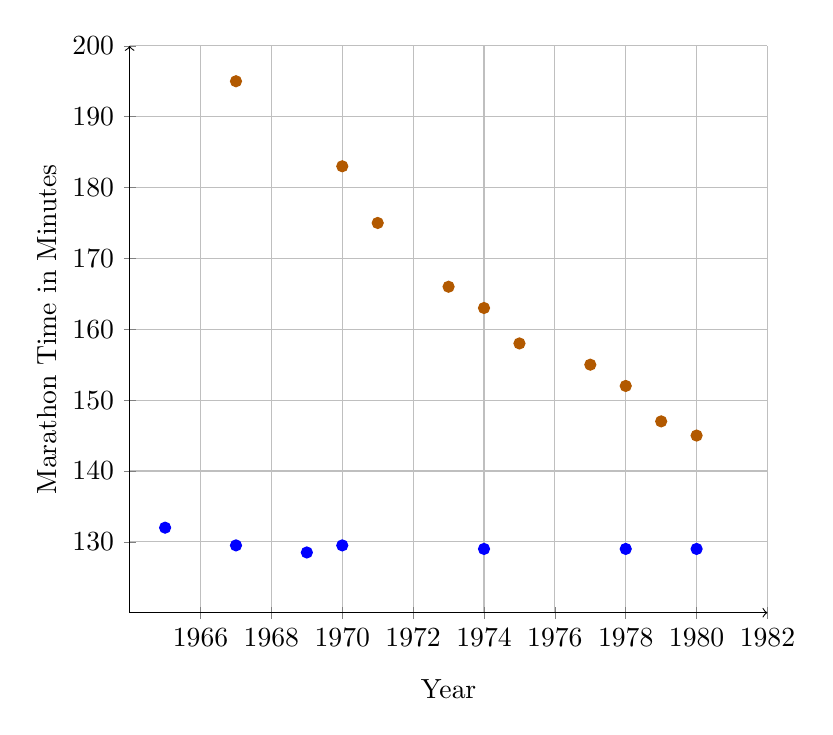
\begin{tikzpicture}
\begin{axis}[
    xmin=0, xmax=18,
    ymin=0, ymax=80,
    axis lines=center,
    axis on top=false,
    domain=0:1,
    x=0.45cm,
    y=0.09cm,
    xtick={0,2,...,18},
    xticklabels={1964,1966,1968,1970,1972,1974,1976,1978,1980,1982},
    ytick={0,10,...,80},
    yticklabels={120,130,140,150,160,170,180,190,200},
    axis lines=middle,
    axis line style={->},
    x label style={at={(axis description cs:0.5,-0.1)},anchor=north},
    y label style={at={(axis description cs:-0.1,.5)},rotate=90,anchor=south},
    xlabel={Year},
    ylabel={Marathon Time in Minutes},
    grid=major
    ]
	\addplot [blue,only marks] table {
	1 12
	3 9.5
	5 8.5
	6 9.5
	10 9
	14 9
	16 9
	};
	\addplot [orange!70!black,only marks] table {
	3 75
	6 63
	7 55
	9 46
	10 43
	11 38
	13 35
	14 32
	15 27
	16 25
	};
	%\addplot [blue, thick] table {
	
	%};
\end{axis}
\end{tikzpicture}
%\includegraphics[width=\textwidth]{MarathonTimes1}
\end{center}
\pagebreak

From this data, it looks like both sets of data are following a linear trend.  If we use the first and last data points to find the average rate of change for each, we get the following linear models, using 1967 as $t=0$:
\begin{align*}
M_t &= 129.5-0.2t\\
W_t &= 195-3.85t
\end{align*}

According to these two linear models, we would predict that the women's record would beat the men's record by 1985; however, in 1985, the men's record was still 14 minutes faster than the women's.  What happened here?\\

Since women began setting marathon records about 50 years later than men, in the early years their progress was drastic, but eventually slowed down, and the trend was not linear over the long run (wow, what a terrible pun).\\

It should be clear that this linear trend was misleading, since if we extrapolated this model too far forward, we'd get ridiculous results.  The model predicts, for instance, that women would run the marathon in 1:20:00 in 1997 (a pace of about 20 mph, the speed of a roadrunner or close to the top speed of Usain Bolt at full sprint), or that by 2017 they'd be running it in 2.5 minutes (around 630 mph).
\end{example}

The lesson is simple, and hopefully obvious: linear trends are usually only useful in the short term; few phenomena follow linear trends over the long run.  That is why we'll examine other types of models in the coming sections.  However, keep this in mind, because we'll find that even those more sophisticated models have their limitations, and often they too break down in the long run.

\begin{exercises}
\ptwo{Marko currently has 20 tulips in his yard.  Each year he plants 5 more.
\begin{enumerate}[(a)]
\item Write a recursive formula for the number of tulips Marko has.
\item Write an explicit formula for the number of tulips Marko has.
\end{enumerate}
}
\ptwo{Pam is a DJ.  Every week she buys 3 new albums to add to her collection.  She currently owns 450 albums.
\begin{enumerate}[(a)]
\item Write a recursive formula for the number of albums Pam has.
\item Write an explicit formula for the number of albums Pam has.
\end{enumerate}
}

\ptwo{A store's sales (in thousands of dollars) grow according to the recursive rule $P_t = P_{t-1} + 15$, with initial sales $P_0 = 40$.
\begin{enumerate}[(a)]
\item Calculate $P_1$ and $P_2$.
\item Find an explicit formula for $P_t$.
\item Use the explicit formula to predict the store's sales in 10 years.
\item When will the store's sales exceed \$100,000?
\end{enumerate}
}
\ptwo{The number of houses in a town has been growing according to the recursive rule $P_t = P_{t-1} + 30$, with an initial number of $P_0 = 200$.
\begin{enumerate}[(a)]
\item Calculate $P_1$ and $P_2$.
\item Find an explicit formula for $P_t$.
\item Use the explicit formula to predict the number of houses in 10 years.
\item When will the number of houses reach 400?
\end{enumerate}
}

\ptwo{A population of beetles is growing according to a linear growth model.  The initial population (week 0) was $P_0=3$, and the population after 8 weeks is $P_8=67$.
\begin{enumerate}[(a)]
\item Find an explicit formula for the beetle population in week $t$.
\item After how many weeks will the beetle population reach 187?
\end{enumerate}
}
\ptwo{The number of streetlights in a town is growing linearly.  Four months ago ($t=0$) there were 130 lights.  Now ($t=4$) there are 146 lights.  If this trend continues,
\begin{enumerate}[(a)]
\item Find an explicit formula for the number of lights in month $t$.
\item How many months will it take to reach 200 lights?
\end{enumerate}
}
\end{exercises}